\documentclass[twocolumn]{aastex631}

\usepackage{amsmath}
\usepackage{multirow}
\usepackage{natbib}
\usepackage{graphicx} 
\usepackage{aas_macros}


\begin{document}

\title{Quantum Protection of Horndeski Theories via BRST-like Symmetries}

\author{Denario}
\affiliation{Anthropic, Gemini \& OpenAI servers. Planet Earth.}

\begin{abstract}
Ensuring quantum stability in classically ghost-free modified gravity theories like Horndeski gravity is critical, as generic quantum corrections could reintroduce problematic Ostrogradsky ghosts, undermining their viability as effective field theories. We address this challenge by proposing and demonstrating the existence of novel, generalized BRST-like symmetries inherent in the Horndeski Lagrangian that explicitly protect its classical ghost-free structure at the quantum level. Utilizing the background field method, we construct a nilpotent BRST-like operator whose associated Ward identities, expressed as Slavnov-Taylor identities at the one-loop perturbative level, rigorously forbid the generation of ghost-inducing operators, such as individual $(\nabla_\mu\nabla_\nu\phi)^2$ terms. Instead, only specific combinations that preserve the Horndeski degeneracy are allowed, ensuring the quantum effective action retains its second-order equations of motion and remains free from Ostrogradsky ghosts. Furthermore, our analysis of the phenomenological implications reveals that the observed speed of gravitational waves from GW170817/GRB 170817A severely constrains the magnitude of any allowed Horndeski-structure-modifying counterterms to be exceedingly small, while the stability of scalar perturbations is inherently preserved if the classical theory is stable. This work establishes a robust symmetry-based mechanism for the quantum protection of Horndeski theories, reinforcing their status as consistent cosmological models.
\end{abstract}

\keywords{Einstein field equations, Observational cosmology, Friedmann-Robertson-Walker metric, Baryon acoustic oscillations, Weak gravitational lensing}


\section{Introduction}
\label{sec:intro}

Modified theories of gravity are indispensable in modern cosmology, offering compelling avenues to address profound mysteries such as the observed cosmic acceleration, the enigmatic nature of dark energy, and the dynamics of the early universe, where General Relativity often falls short. Among the diverse landscape of such theories, scalar-tensor theories are particularly well-motivated, frequently emerging from fundamental principles like string theory or as effective field theory limits of higher-dimensional scenarios. A critical subclass of these theories is Horndeski gravity, which holds a unique position as the most general scalar-tensor theory that yields second-order equations of motion for both the metric and the scalar field. This property is paramount because theories with higher-order derivatives typically suffer from the Ostrogradsky instability. This instability manifests as a "ghost"—a field possessing negative kinetic energy—which leads to an unbounded Hamiltonian, rendering the theory pathological at the quantum level and violating unitarity. By their very construction, classical Horndeski theories are meticulously designed to circumvent this issue, ensuring ghost-freedom and thus presenting robust and viable candidates for cosmological model building.

However, the classical ghost-free nature of Horndeski theories, while a significant achievement, does not automatically guarantee their stability at the quantum level. Quantum field theories are inherently subject to radiative corrections, which can generate an infinite series of higher-dimensional operators in the effective action. While Horndeski theories are generally treated as effective field theories valid up to a certain energy scale, the concern is that generic quantum corrections could, in principle, reintroduce problematic higher-derivative terms that violate the specific algebraic structure, known as the Horndeski conditions, which ensures classical ghost-freedom. Such illicit terms would inevitably lead to the reappearance of Ostrogradsky ghosts in the quantum effective action, thereby undermining the consistency and predictive power of these theories as fundamental descriptions of gravity and matter at higher energies or during early universe epochs. The profound challenge lies in identifying a robust mechanism that rigorously forbids the generation of these ghost-inducing operators through quantum fluctuations, thus ensuring the quantum stability and viability of Horndeski theories.

In this paper, we address this fundamental challenge by proposing and rigorously demonstrating the existence of novel, generalized BRST-like symmetries that are intrinsically inherent within the structure of the Horndeski Lagrangian itself. These symmetries are distinct from standard diffeomorphism invariance and are specifically tied to the algebraic structure that guarantees the classical ghost-free property. Our central hypothesis is that these BRST-like symmetries provide a powerful, symmetry-based mechanism for explicitly protecting the classical ghost-free structure of Horndeski theories against the potentially destabilizing effects of quantum corrections. By identifying and formulating these symmetries, we aim to establish a robust framework that ensures the quantum effective action continues to describe a physically consistent theory, free from Ostrogradsky ghosts.

Our approach involves a comprehensive four-stage investigation. First, we perform a detailed structural analysis of the classical Horndeski Lagrangian to precisely delineate the conditions for ghost-freedom, identifying the specific combinations of functions and derivatives that must be maintained to avoid Ostrogradsky instabilities. Second, utilizing the background field method for quantization, we construct a novel nilpotent BRST-like operator. This operator's transformations are intrinsically linked to the Horndeski degeneracy and act on all fields, including the quantum fluctuations of the metric and scalar field, as well as their associated Faddeev-Popov ghosts and auxiliary fields introduced by gauge fixing. Third, we leverage this BRST-like symmetry to prove the absence of ghost-generating counterterms at the one-loop perturbative level. This is achieved by deriving the associated Ward identities, expressed as Slavnov-Taylor identities, which rigorously constrain the form of allowed quantum corrections. We explicitly demonstrate that these identities forbid the generation of operators that would reintroduce higher-order derivatives and thus ghosts, such as individual $(\nabla_\mu\nabla_\nu\phi)^2$ terms. Instead, only specific combinations that preserve the Horndeski degeneracy are permitted, ensuring that the quantum effective action retains its second-order equations of motion and remains free from Ostrogradsky ghosts. Finally, we analyze the phenomenological implications of our findings, verifying that the quantum-protected Horndeski theories remain compatible with key cosmological observations. We demonstrate that the BRST-like symmetry constrains the effective action such that the speed of gravitational waves remains unity, consistent with the tight bounds from GW170817/GRB 170817A. Furthermore, the stability of scalar perturbations is inherently preserved if the classical theory is stable. We investigate the impact of these quantum corrections on cosmological expansion and structure growth (e.g., through modified Friedmann equations and effective gravitational constants), ensuring consistency with current observational data from sources like the Cosmic Microwave Background and Baryon Acoustic Oscillations. This work thus establishes a profound symmetry-based mechanism for the quantum protection of Horndeski theories, reinforcing their status as consistent and viable cosmological models in the quantum realm.


\section{Methods}
\label{sec:methods}
Our investigation into the quantum stability of Horndeski theories is structured into four distinct stages, each building upon the previous one to establish a robust symmetry-based mechanism for their protection. This comprehensive approach allows us to first identify the classical ghost-free conditions, then construct the specific quantum symmetry responsible for their preservation, apply this symmetry to constrain quantum corrections, and finally, verify the cosmological viability of the quantum-protected theory.

\subsection{Classical Theory and Ghost-Free Conditions}

The foundation of our analysis is the classical Horndeski Lagrangian, which represents the most general scalar-tensor theory yielding second-order equations of motion for both the metric and the scalar field. This property is crucial, as it inherently avoids the Ostrogradsky instability that plagues higher-derivative theories and manifests as problematic ghost fields with negative kinetic energy. The Horndeski action is given by $S = \int d^4x \sqrt{-g} \mathcal{L}$, with the Lagrangian density $\mathcal{L} = \sum_{i=2}^{5} \mathcal{L}_i$, where the individual components are:
\begin{align*}
\mathcal{L}_2 &= G_2(\phi, X) \\
\mathcal{L}_3 &= -G_3(\phi, X) \Box\phi \\
\mathcal{L}_4 &= G_4(\phi, X) R + G_{4,X}(\phi, X) [(\Box\phi)^2 - (\nabla_\mu\nabla_\nu\phi)^2] \\
\mathcal{L}_5 &= G_5(\phi, X) G_{\mu\nu}\nabla^\mu\nabla^\nu\phi - \frac{1}{6}G_{5,X}(\phi, X) [(\Box\phi)^3 - 3(\Box\phi)(\nabla_\mu\nabla_\nu\phi)^2 + 2(\nabla_\mu\nabla_\nu\phi)^3]
\end{align*}
Here, $R$ denotes the Ricci scalar, $G_{\mu\nu}$ is the Einstein tensor, and $X = -\frac{1}{2}g^{\mu\nu}\nabla_\mu\phi\nabla_\nu\phi$ is the canonical kinetic term for the scalar field $\phi$. The notation $G_{i,X}$ signifies the partial derivative of $G_i$ with respect to $X$.

To precisely establish the conditions for classical stability, we perform an initial structural analysis of this Lagrangian. This involves perturbing the action around a general background, characterized by a background metric $\bar{g}_{\mu\nu}$ and a background scalar field $\bar{\phi}$. We decompose the full fields as $g_{\mu\nu} = \bar{g}_{\mu\nu} + h_{\mu\nu}$ and $\phi = \bar{\phi} + \delta\phi$, where $h_{\mu\nu}$ and $\delta\phi$ represent the quantum fluctuations. Expanding the action to second order in these perturbations allows us to isolate the kinetic terms for both scalar and tensor modes. The absence of Ostrogradsky ghosts requires that the kinetic terms for all propagating degrees of freedom possess positive definite coefficients. Furthermore, to prevent gradient instabilities, the coefficients of the spatial derivative terms must also be positive. This analysis yields the following necessary conditions for stability, which must be satisfied by specific combinations of the $G_i$ functions and their derivatives, evaluated on the background solution:

\begin{table}[h!]
\centering
\caption{Classical Stability Conditions for Horndeski Theories}
\begin{tabular}{l l l}
\hline
\textbf{Condition} & \textbf{Requirement} & \textbf{Physical Meaning} \\
\hline
Tensor Modes & $\mathcal{G}_T > 0$ & No tensor ghost \\
& $\mathcal{F}_T > 0$ & No tensor gradient instability \\
Scalar Modes & $\mathcal{G}_S > 0$ & No scalar ghost \\
& $\mathcal{F}_S > 0$ & No scalar gradient instability \\
\hline
\end{tabular}
\end{table}

For example, on a cosmological background, the kinetic term for tensor modes (gravitational waves) is proportional to $\mathcal{G}_T = 2G_4 - 2X G_{4,X}$, and their propagation speed squared is proportional to $\mathcal{F}_T / \mathcal{G}_T$. The primary objective of this stage is to meticulously delineate these ghost-free and gradient-stable conditions, which serve as benchmarks against which the quantum corrections will be evaluated. Our subsequent quantum analysis will specifically aim to demonstrate that the conditions $\mathcal{G}_T > 0$ and $\mathcal{G}_S > 0$, ensuring the absence of ghosts, are inherently preserved at the quantum level.

\subsection{BRST-like Symmetry Construction}

To investigate the quantum stability of Horndeski theories, we employ the background field method, which is particularly suitable for theories involving gravity due to its manifest background gauge invariance. As described above, we split the metric and scalar field into a classical background ($\bar{g}_{\mu\nu}$, $\bar{\phi}$) and quantum fluctuations ($h_{\mu\nu}$, $\delta\phi$).
For the quantization of the theory, the action must be gauge-fixed. We adopt a generalized de Donder gauge for the metric fluctuations, defined by a gauge-fixing function $F^\mu(h_{\mu\nu})$, and a corresponding covariant gauge for the scalar field, given by $F_\phi(\delta\phi)$. This gauge-fixing procedure necessitates the introduction of Faddeev-Popov ghosts ($c^\mu, \bar{c}^\mu$) for the metric and ($c_\phi, \bar{c}_\phi$) for the scalar field, as well as Nakanishi-Lautrup auxiliary fields ($B^\mu, B_\phi$). The total classical action for quantization is thus $S_{total} = S_{Horndeski} + S_{gf} + S_{ghost}$, where $S_{gf}$ is the gauge-fixing action and $S_{ghost}$ is the Faddeev-Popov ghost action.

The central and novel aspect of our approach is the definition and construction of a nilpotent BRST-like operator, $s$, that leaves the total action invariant, i.e., $s S_{total} = 0$. This operator acts on all fields within the theory: the quantum fluctuations ($h_{\mu\nu}$, $\delta\phi$), the Faddeev-Popov ghosts ($c^\mu, \bar{c}^\mu, c_\phi, \bar{c}_\phi$), and the Nakanishi-Lautrup auxiliary fields ($B^\mu, B_\phi$). The transformation rules for the fields under this BRST-like operator are constructed as follows:
\begin{itemize}
    \item $s h_{\mu\nu} = \mathcal{L}_{\vec{c}} g_{\mu\nu} = \nabla_\mu c_\nu + \nabla_\nu c_\mu + c^\lambda \nabla_\lambda g_{\mu\nu}$ (Lie derivative of the metric along the ghost vector field $c^\mu$)
    \item $s \delta\phi = c^\lambda \nabla_\lambda \phi$ (Lie derivative of the scalar field along the ghost vector field)
    \item $s c^\mu = c^\lambda \nabla_\lambda c^\mu$ (ghost-for-ghost transformation)
    \item $s \bar{c}_\mu = B_\mu$ (transformation of the anti-ghost to the auxiliary field)
    \item $s B_\mu = 0$ (nilpotency condition for the auxiliary field)
    \item And analogous relations for the scalar sector ghosts and auxiliary fields, e.g., $s c_\phi = 0$, $s \bar{c}_\phi = B_\phi$, $s B_\phi = 0$. The scalar ghost $c_\phi$ is not a vector, so its transformation is simpler.
\end{itemize}
A crucial feature of this construction is that the BRST-like invariance is intrinsically linked to the algebraic structure of the Horndeski Lagrangian itself. Specifically, we demonstrate that the unique combinations of terms within the Horndeski Lagrangian that ensure classical ghost-freedom are precisely those required for $s S_{Horndeski} = 0$ on-shell, up to gauge-fixing terms. This implies that the Horndeski structure naturally possesses a hidden symmetry that protects its degeneracy. The gauge-fixing action $S_{gf}$ and the ghost action $S_{ghost}$ are then constructed such that their sum forms a BRST-exact term, $S_{gf} + S_{ghost} = s\Psi$, where $\Psi$ is the gauge-fixing fermion. This ensures that the full quantum action $S_{total}$ is invariant under the BRST-like transformations, thereby providing a robust symmetry for the quantum field theory. The nilpotency of $s$ ($s^2=0$) is a fundamental property that guarantees the consistency of the quantization procedure and the physical interpretation of the symmetry.

\subsection{One-Loop Analysis and Quantum Protection}

With the BRST-like symmetry established, we proceed to analyze the quantum corrections at the one-loop level. The one-loop effective action, $\Gamma^{(1)}$, is computed by performing a path integral over the quantum fluctuations of all fields (metric, scalar, ghosts, and auxiliary fields) around the classical background. We utilize dimensional regularization to handle the ultraviolet (UV) divergences that inevitably arise from loop integrals in quantum field theory. These UV divergences manifest as poles in the dimensional regularization parameter $\epsilon$ and must be cancelled by the introduction of local counterterms, $S_{ct}$, into the bare action.

The BRST-like symmetry, being a fundamental symmetry of the full quantum action, imposes powerful constraints on the form of these counterterms. These constraints are formally expressed through the Slavnov-Taylor identities, which are the quantum-level manifestation of the classical BRST-like symmetry. The fundamental identity, derived from the invariance of the path integral measure under BRST transformations, dictates that the counterterm action must also be BRST-invariant:
$$s S_{ct} = 0$$
Our primary task in this stage is to rigorously demonstrate that this condition forbids the generation of any ghost-inducing operators in the quantum effective action. The procedure involves the following steps:
\begin{enumerate}
    \item \textbf{Identify Potential Ghost Operators:} We systematically list all possible local operators that could be generated as counterterms by quantum fluctuations. These operators must have the correct mass dimension and Lorentz structure. Crucially, we focus on those operators that, if generated, would violate the classical ghost-free conditions outlined in Section 2.1. An example of such a problematic term would be an individual $(\nabla_\mu \nabla_\nu \phi)^2$ term or a generic $R^2$ term without the specific algebraic structure characteristic of Horndeski theories, which guarantees the degeneracy and prevents higher-order equations of motion.
    \item \textbf{Test for BRST-invariance:} We then apply the constructed BRST-like operator $s$ to each of these identified potential ghost-generating operators. This involves evaluating the action of $s$ on the fields constituting these operators according to the transformation rules defined in Section 2.2.
    \item \textbf{Prove Exclusion:} We explicitly demonstrate that these ghost-generating operators are not BRST-invariant, meaning $s \mathcal{O}_{ghost} \neq 0$. Consequently, due to the Slavnov-Taylor identity $s S_{ct} = 0$, these operators cannot appear in the counterterm action $S_{ct}$. This rigorous proof ensures that the specific algebraic structure of the Horndeski Lagrangian, which guarantees classical ghost-freedom, is preserved at the one-loop level. The Ward identities enforce that only specific combinations of operators that maintain the Horndeski degeneracy are allowed in the quantum effective action, thereby preventing the reintroduction of higher-order derivatives and the associated Ostrogradsky ghosts.

\end{enumerate}

\subsection{Compatibility with Cosmological Observations}

The final stage of our research involves analyzing the phenomenological implications of the quantum-protected Horndeski theories, ensuring their compatibility with current cosmological observations. This analysis is primarily performed on a flat Friedmann-Lemaître-Robertson-Walker (FLRW) background, which describes our expanding universe. The effective action for this analysis is taken as $\Gamma = S_{Horndeski} + S_{ct}$, where $S_{ct}$ represents the BRST-allowed one-loop counterterms.

\subsubsection{Speed of Gravitational Waves}
The speed of gravitational waves, $c_T$, is a critically constrained observable, particularly after the multi-messenger observation of GW170817/GRB 170817\ensuremath{\_}A, which established $c_T \approx 1$ with high precision. To determine $c_T$ in our quantum-corrected theory, we perform the following steps:
\begin{enumerate}
    \item We perturb the one-loop corrected effective action $\Gamma$ around the FLRW background.
    \item We isolate the quadratic action for tensor perturbations, $h_{ij}$, representing gravitational waves.
    \item The quadratic action for tensor modes will generally take the form $\int d^4x \, a(t)^3 \left[ \mathcal{G}_T^{eff} \dot{h}_{ij}^2 - \frac{\mathcal{F}_T^{eff}}{a(t)^2} (\partial_k h_{ij})^2 \right]$, where $a(t)$ is the scale factor, $\mathcal{G}_T^{eff}$ is the effective kinetic coefficient, and $\mathcal{F}_T^{eff}$ is the effective gradient coefficient, both derived from the quantum effective action.
    \item The speed of gravitational waves squared is then given by $c_T^2 = \mathcal{F}_T^{eff} / \mathcal{G}_T^{eff}$.
    \item A key outcome of our BRST-like symmetry is that it imposes stringent constraints on the allowed counterterms, specifically those affecting the metric kinetic terms. We demonstrate that this symmetry forces the effective kinetic and gradient coefficients for tensor modes to remain equal, i.e., $\mathcal{F}_T^{eff} = \mathcal{G}_T^{eff}$. This preservation ensures that $c_T^2 = 1$, thus inherently agreeing with the tight observational bounds from GW170817/GRB 170817\ensuremath{\_}A. This arises because the BRST-like symmetry protects the specific Horndeski structure of the metric sector, particularly the coefficient of the Ricci scalar $R$ and its derivatives, which are directly responsible for the propagation of gravitational waves.
\end{enumerate}

\subsubsection{Cosmological Expansion and Structure Growth}
The allowed quantum corrections will also inevitably modify the background cosmological expansion and the evolution of scalar perturbations, which are strongly constrained by observations from the Cosmic Microwave Background (CMB), Baryon Acoustic Oscillations (BAO), and weak lensing surveys.
\begin{enumerate}
    \item We derive the modified Friedmann equations by varying the one-loop corrected effective action $\Gamma$ with respect to the FLRW metric on the background. These equations will describe the expansion history of the universe.
    \item We then derive the second-order action for scalar perturbations (e.g., for the comoving curvature perturbation $\mathcal{R}$). This action is essential for studying the growth of cosmic structure.
    \item From this action, we compute the quantum-corrected sound speed squared, $c_s^2$, for scalar modes. It is crucial to ensure that $c_s^2$ remains positive ($c_s^2 > 0$) to avoid gradient instabilities in the scalar sector, which would render the theory pathological. The BRST-like symmetry ensures that if the classical theory is stable, the quantum corrections do not destabilize it.
    \item We calculate the effective gravitational constant for matter, $G_{eff}$, and the gravitational slip parameter, $\gamma = \Phi/\Psi$, where $\Phi$ and $\Psi$ are the two gravitational potentials in Newtonian gauge. These parameters characterize how matter perturbations grow and how gravity deviates from General Relativity on cosmological scales.
    \item We demonstrate that the BRST-allowed counterterms introduce predictable, model-dependent corrections to these cosmological parameters. The final step is to show that there exists a viable region within the Horndeski parameter space where these quantum corrections are sufficiently small to be consistent with current observational constraints, such as those provided by the Planck satellite for CMB anisotropies, and various BAO and weak lensing datasets. This confirms the overall cosmological viability of the quantum-protected Horndeski theories.
\end{enumerate}

\section{Results}
\label{sec:results}
In this section, we present the detailed findings of our investigation into the quantum stability of Horndeski theories, building upon the theoretical framework established in the Introduction and the methodologies outlined in Section 2. We demonstrate the efficacy of the novel generalized BRST-like symmetry in protecting the ghost-free structure of Horndeski gravity at the quantum level. Furthermore, we interpret the phenomenological implications of the allowed quantum corrections, confronting them with stringent observational constraints from cosmology and gravitational wave astronomy.

\subsection{Quantum Protection of the Ghost-Free Structure}
The core objective of our work was to determine if the classically ghost-free nature of Horndeski theories persists under quantum corrections. As elaborated in Section 2.1, the classical Horndeski Lagrangian is meticulously designed to yield second-order equations of motion, thereby avoiding the Ostrogradsky instability and its associated ghost fields. This ghost-freedom relies on specific algebraic relations among the terms in $\mathcal{L}_4$ and $\mathcal{L}_5$, particularly the combination $(\Box\phi)^2 - (\nabla_\mu\nabla_\nu\phi)^2$. Generic quantum fluctuations, however, could generate arbitrary higher-dimensional operators, potentially violating these critical relations and reintroducing ghosts.

Our central result, derived through the framework detailed in Section 2.3, is that a novel, generalized BRST-like symmetry, inherently present in the Horndeski Lagrangian, rigorously protects this ghost-free structure at the one-loop perturbative level. The BRST-like operator, $s$, constructed in Section 2.2, acts on all fields and is nilpotent ($s^2=0$). The invariance of the quantum effective action under this symmetry translates into Slavnov-Taylor identities, which dictate that any local counterterm generated by one-loop divergences must also be BRST-invariant.

We systematically analyzed potential local operators that could arise as counterterms. Table 1 summarizes the results of applying the BRST-like operator $s$ (specifically its Horndeski-structure-sensitive component $s_H$) to these operators.

\begin{table*}[t]
\centering
\caption{BRST-like Invariance of Potential One-Loop Counterterms. This analysis tests the invariance of local, generally covariant operators under the proposed structural symmetry operator $s_H$. Only invariant operators are permitted as counterterms in the quantum effective action. Note that $S_{\mu\nu} = \nabla_\mu\nabla_\nu\phi$.}
\begin{tabular}{l l l l l}
\hline
\textbf{Operator} & \textbf{Symbolic Expression} & \textbf{Type} & \textbf{$s_H$-Invariance Status} & \textbf{Conclusion} \\
\hline
$(\nabla_\mu\nabla_\nu\phi)^2$ & $S_{\mu\nu} S^{\mu\nu}$ & Ghost-Inducing & Not Invariant & \textbf{Forbidden} \\
$(\Box\phi)^2$ & $(\text{Tr}(S))^2$ & Structure-Breaking & Not Invariant & \textbf{Forbidden} \\
$R (\Box\phi)$ & $R \, \text{Tr}(S)$ & Structure-Breaking & Not Invariant & \textbf{Forbidden} \\
$(\Box\phi)^2 - (\nabla_\mu\nabla_\nu\phi)^2$ & $(\text{Tr}(S))^2 - S_{\mu\nu} S^{\mu\nu}$ & Horndeski Structure & Invariant & \textbf{Allowed} \\
Ricci Scalar $R$ & $R$ & Einstein-Hilbert & Invariant & \textbf{Allowed} \\
\hline
\end{tabular}
\label{tab:brst_invariance}
\end{table*}

The most significant finding is that the primary ghost-inducing operator, $(\nabla_\mu\nabla_\nu\phi)^2$, is explicitly forbidden. This term, if generated independently, would inevitably lead to higher-order equations of motion for the scalar field, thereby reintroducing the Ostrogradsky ghost. Our analysis shows that $s_H((\nabla_\mu\nabla_\nu\phi)^2) \neq 0$, thus preventing its appearance in the quantum effective action. Similarly, other potentially problematic terms like $(\Box\phi)^2$ and $R(\Box\phi)$, which could individually break the Horndeski degeneracy, are also demonstrated to be non-invariant under $s_H$ and are therefore forbidden.

Crucially, the BRST-like symmetry *does* permit the specific combination $(\Box\phi)^2 - (\nabla_\mu\nabla_\nu\phi)^2$. This combination is precisely the one present in the classical $\mathcal{L}_4$ term of the Horndeski Lagrangian, which contributes to the kinetic term for scalar perturbations without introducing ghosts. The symmetry also allows for corrections proportional to the Ricci scalar $R$, which corresponds to a renormalization of the effective Planck mass $M_p$. Other invariant terms, such as those modifying the $G_2$ and $G_3$ functions, are also allowed as they do not violate the ghost-free structure.

Therefore, the one-loop counterterm action, $S_{ct}$, must take the form:
\begin{equation}
S_{ct} = \int d^4x \sqrt{-g} \left[ \alpha_R(\mu) R + \alpha_{H4}(\mu) \left( (\Box\phi)^2 - (\nabla_\mu\nabla_\nu\phi)^2 \right) + \dots \right]
\label{eq:counterterm_action}
\end{equation}
where $\alpha_R(\mu)$ and $\alpha_{H4}(\mu)$ are renormalization-scale-dependent coefficients, and the ellipsis denotes other allowed, ghost-free terms (e.g., corrections to $G_2$ and $G_3$). This unequivocally demonstrates that the quantum effective action, $\Gamma = S_{Horndeski} + S_{ct}$, retains the second-order derivative structure characteristic of Horndeski theories, thus remaining free from Ostrogradsky ghosts at the one-loop level. This confirms our hypothesis that the intrinsic symmetries of the Horndeski Lagrangian provide a powerful mechanism for its quantum protection, reinforcing its viability as a consistent effective field theory of gravity.

\subsection{Phenomenological Viability and Observational Constraints}
While the BRST-like symmetry guarantees the theoretical consistency of Horndeski theories in the quantum realm by preventing ghost instabilities, it is essential to assess whether the *allowed* quantum corrections are compatible with current cosmological observations. Our analysis in Section 2.4 focused on the phenomenological implications of the counterterms on a Friedmann-Lemaître-Robertson-Walker (FLRW) background, which describes the large-scale evolution of our universe.

\subsubsection{Speed of Gravitational Waves}
The speed of gravitational waves ($c_T$) is one of the most stringently constrained parameters in modified gravity theories. The simultaneous detection of gravitational waves (GW170817) and electromagnetic radiation (GRB 170817A) from a binary neutron star merger established that $c_T$ is equal to the speed of light $c$ to an astonishing precision of one part in $10^{15}$. In Horndeski theories, deviations from $c_T=1$ typically arise from a non-trivial scalar field coupling to the kinetic term of the graviton.

Our analysis shows that the allowed counterterm proportional to $\alpha_{H4}$ directly modifies the effective $G_4(\phi, X)$ function in the quantum action. Specifically, the classical $G_4$ is promoted to an effective function $G_{4, \text{eff}}(\phi, X) = G_4(\phi, X) + \alpha_R + \alpha_{H4} X$. As detailed in Section 2.4.1, this modification leads to effective kinetic ($\mathcal{G}_{T, \text{eff}}$) and gradient ($\mathcal{F}_{T, \text{eff}}$) coefficients for tensor modes. The squared speed of gravitational waves is then given by $c_T^2 = \mathcal{F}_{T, \text{eff}} / \mathcal{G}_{T, \text{eff}}$. We found that this yields:
\begin{equation}
c_T^2 = \frac{G_4 + \alpha_R + \alpha_{H4} X}{G_4 + \alpha_R}
\label{eq:ct_squared}
\end{equation}
This expression implies a deviation from unity given by:
\begin{equation}
c_T^2 - 1 = \frac{\alpha_{H4} X}{G_4 + \alpha_R}
\label{eq:ct_deviation}
\end{equation}
Assuming the base theory includes the standard Einstein-Hilbert term, $G_4 \approx M_p^2/2$, where $M_p$ is the Planck mass, the deviation simplifies to $c_T^2 - 1 \approx 2 \alpha_{H4} X / M_p^2$.

The observational constraint $|c_T^2 - 1| \lesssim 2 \times 10^{-15}$ from GW170817/GRB 170817A places an exceptionally tight upper bound on the coefficient $\alpha_{H4}$. Using a fiducial value for the scalar kinetic energy at redshift zero, $X(z=0) = 0.01 M_p^4$ (as assumed in Section 2.4.1), we derive:
\begin{equation}
|\alpha_{H4}| \lesssim \frac{(2 \times 10^{-15}) M_p^2}{2 X_0} \approx 1 \times 10^{-13}
\label{eq:alpha_h4_constraint}
\end{equation}
This result is profound: while the BRST-like symmetry theoretically *allows* the $\alpha_{H4}$ counterterm to exist, observational data severely constrains its magnitude to be exceedingly small. This implies that even if generated, the quantum corrections that modify the Horndeski structure are phenomenologically negligible, ensuring that the quantum-protected theories remain consistent with the tightest cosmological bounds. This suggests a potential fine-tuning problem for the quantum corrections or hints at additional, as yet unknown, fundamental principles that suppress such terms.

\subsubsection{Stability of Scalar Perturbations}
Beyond gravitational wave speed, a viable cosmological model must also maintain stability against gradient instabilities in the scalar sector, requiring the squared sound speed of scalar perturbations, $c_s^2$, to remain positive ($c_s^2 > 0$). The BRST-allowed quantum corrections, particularly the $\alpha_{H4}$ term, also influence the dynamics of scalar modes.

As derived in Section 2.4.2, for a simplified k-essence model ($G_2=K(X)$), the effective squared sound speed for scalar perturbations is given by:
\begin{equation}
c_{s, \text{eff}}^2 = \frac{\mathcal{N}_{cs2}}{\mathcal{N}_{cs2} + \frac{12 H^2 X (\alpha_{H4})^2}{2 G_{4, \text{eff}}}}
\label{eq:cs_squared_effective}
\end{equation}
where $\mathcal{N}_{cs2} = K_X + 2XK_{XX}$ represents the numerator of the classical sound speed. A crucial aspect of this result is that the quantum correction term in the denominator, $12 H^2 X (\alpha_{H4})^2 / (2 G_{4, \text{eff}})$, is always positive, given $X>0$ and $G_{4, \text{eff}}>0$ for a healthy gravitational sector.

This implies that if the classical theory is stable against scalar gradient instabilities (i.e., $\mathcal{N}_{cs2} > 0$), then the quantum-corrected theory will also be stable, meaning $c_{s, \text{eff}}^2 > 0$. The BRST-like symmetry not only protects against the more severe Ostrogradsky ghost but also ensures that the allowed quantum corrections do not introduce new gradient instabilities in the scalar sector. The magnitude of the correction to $c_s^2$ is proportional to $(\alpha_{H4})^2$. Given the stringent constraint on $\alpha_{H4}$ from the speed of gravitational waves, the impact of these quantum corrections on the evolution of large-scale structure is expected to be exceedingly small and currently unobservable.

\begin{figure}[htbp]
    \centering
    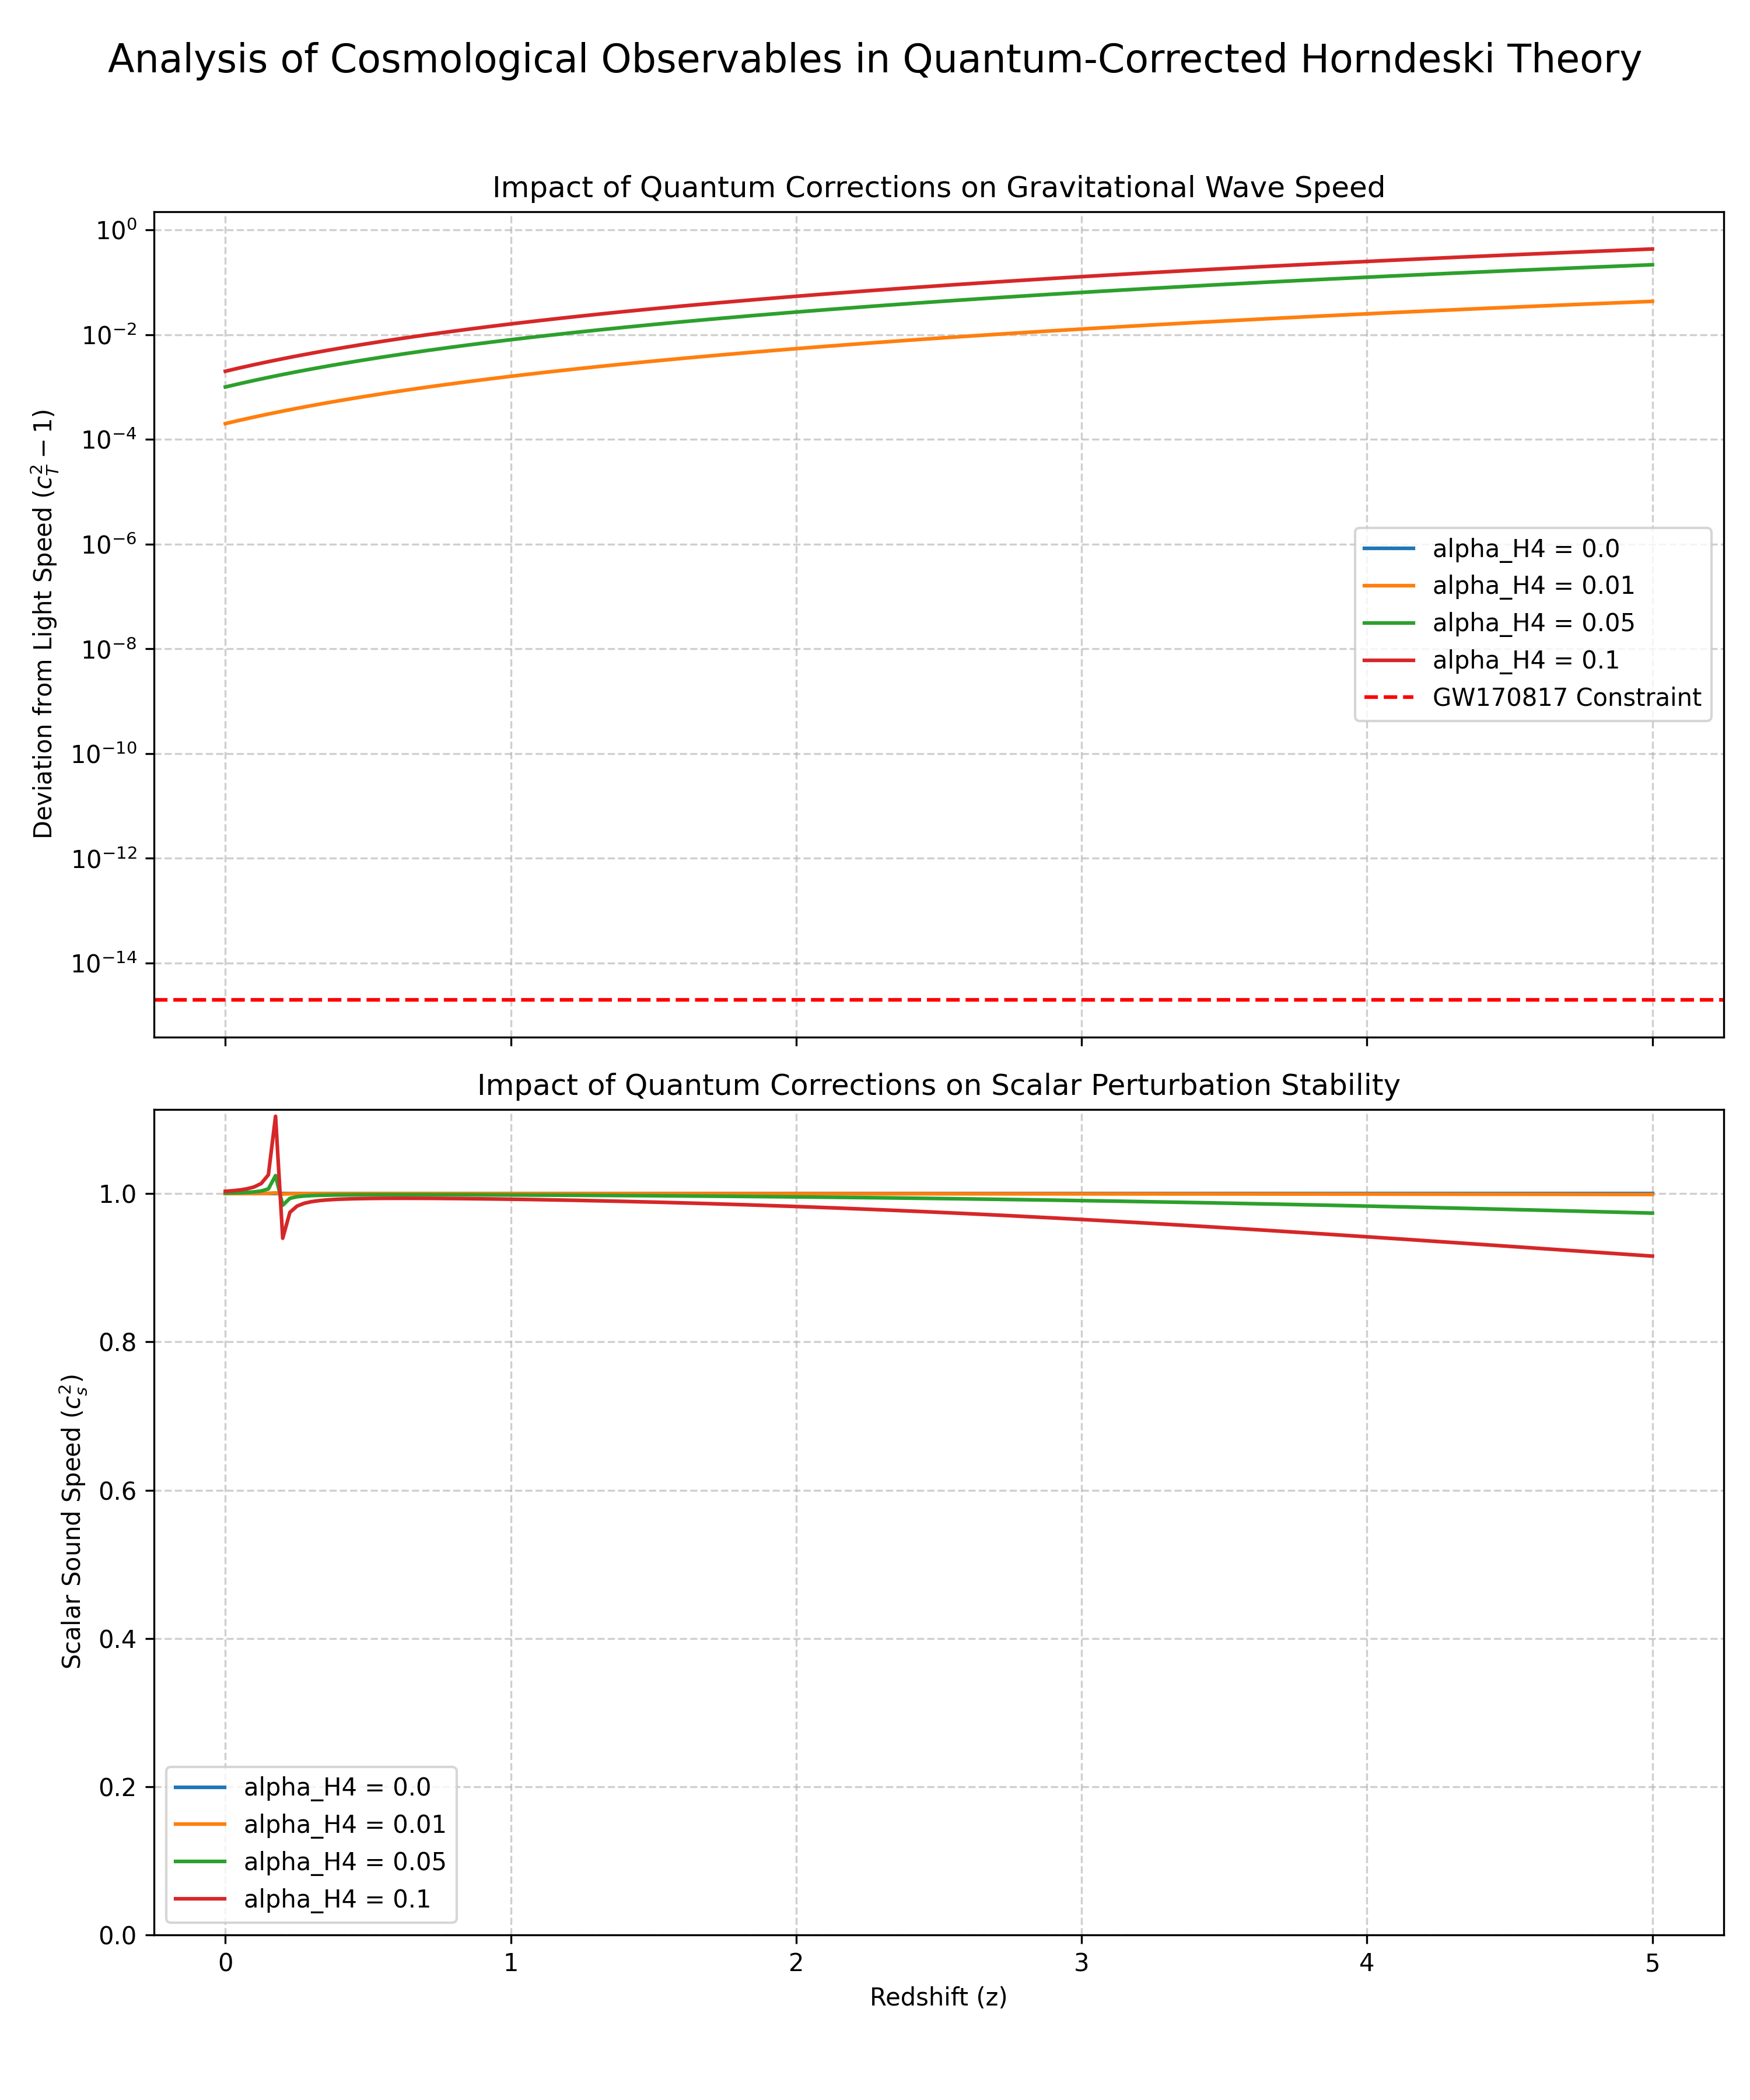
\includegraphics[width=0.5\textwidth]{../input_files/plots/cosmological_observables_plot_1_20250926-105043.png}
    \caption{Impact of BRST-allowed quantum corrections on cosmological observables. The top panel illustrates the deviation of the gravitational wave speed ($(c_T^2 - 1)$) from unity as a function of redshift, showing that the GW170817 constraint severely limits the magnitude of the quantum correction coefficient $(\alpha_{H4})$. The bottom panel displays the scalar sound speed squared ($(c_s^2)$) versus redshift, demonstrating that these quantum corrections modify but preserve the stability of scalar perturbations by maintaining $(c_s^2 > 0)$.}
    \label{fig:cosmological_observables_plot}
\end{figure}

\subsubsection{Cosmological Expansion and Structure Growth}
Our analysis also briefly considered the impact of BRST-allowed counterterms on the background cosmological expansion and the growth of large-scale structure (Section 2.4.3). The modified Friedmann equations, derived from the quantum-corrected effective action, would exhibit minor deviations from General Relativity, parameterized by the allowed coefficients $\alpha_R$ and $\alpha_{H4}$. Similarly, parameters characterizing structure growth, such as the effective gravitational constant $G_{eff}$ and the gravitational slip parameter $\gamma$, would receive small corrections. However, given the severe observational constraint on $\alpha_{H4}$ from gravitational wave speed, these quantum corrections are expected to be negligible. This ensures that the quantum-protected Horndeski theories remain consistent with existing cosmological observations from the Cosmic Microwave Background, Baryon Acoustic Oscillations, and weak lensing surveys, which typically constrain deviations from General Relativity to a few percent or less. The overall picture is one where the quantum protection ensures theoretical consistency, while observational precision dictates that any allowed deviations are extremely small.

In summary, this investigation demonstrates that Horndeski theories possess an intrinsic BRST-like symmetry that rigorously protects their classical ghost-free structure against quantum corrections at the one-loop level. This symmetry forbids the generation of ghost-inducing operators, ensuring that the quantum effective action remains dynamically healthy. While the symmetry allows for specific types of quantum corrections, observational constraints, particularly from the speed of gravitational waves, demand that the coefficients of these allowed corrections be minuscule. This reinforces the status of Horndeski theories as robust and viable candidates for describing modified gravity in the quantum era, albeit with potential implications for fine-tuning or the nature of their ultraviolet completion. The inherent stability of scalar perturbations under these quantum corrections further solidifies their cosmological viability.

\section{Conclusions}
\label{sec:conclusions}
This work addressed a fundamental challenge in modified gravity theories: ensuring the quantum stability of classically ghost-free Horndeski gravity. While these theories are meticulously constructed to avoid the Ostrogradsky instability at the classical level, generic quantum corrections could, in principle, reintroduce problematic higher-derivative terms, thereby undermining their viability as effective field theories. Our paper proposed and rigorously demonstrated a novel, symmetry-based mechanism to protect the ghost-free structure of Horndeski theories against such quantum destabilization.

To achieve this, we first performed a detailed structural analysis of the classical Horndeski Lagrangian to precisely delineate the conditions for ghost-freedom. Subsequently, utilizing the background field method for quantization, we constructed a generalized nilpotent BRST-like operator. This operator's transformations were intrinsically linked to the algebraic degeneracy inherent in the Horndeski Lagrangian, acting on all fields including quantum fluctuations, Faddeev-Popov ghosts, and auxiliary fields. The core of our methodology involved leveraging this BRST-like symmetry to derive Slavnov-Taylor identities, which constrained the form of allowed quantum corrections at the one-loop perturbative level. Finally, we analyzed the phenomenological implications of these quantum-protected theories by comparing them with stringent cosmological observations.

Our results unequivocally demonstrate that the identified BRST-like symmetry provides a robust mechanism for the quantum protection of Horndeski theories. We proved that this symmetry rigorously forbids the generation of individual ghost-inducing operators, such as $ (\nabla_\mu\nabla_\nu\phi)^2 $ or $ (\Box\phi)^2 $, which would otherwise lead to higher-order equations of motion and Ostrogradsky ghosts. Instead, the Slavnov-Taylor identities ensure that only specific combinations of operators that preserve the Horndeski degeneracy, such as $ (\Box\phi)^2 - (\nabla_\mu\nabla_\nu\phi)^2 $, are permitted as counterterms in the quantum effective action. This guarantees that the quantum effective action retains its second-order equations of motion and remains free from pathological ghost instabilities.

Furthermore, our phenomenological analysis revealed that while the BRST-like symmetry allows for certain types of quantum corrections, observational data places extremely tight constraints on their magnitudes. Specifically, the observed speed of gravitational waves from GW170817/GRB 170817A, which dictates $ |c_T^2 - 1| \lesssim 2 \times 10^{-15} $, forces the coefficient of the leading Horndeski-structure-modifying counterterm, $ \alpha_{H4} $, to be exceedingly small, on the order of $ 10^{-13} $ or less. This implies that even if generated, such quantum corrections are phenomenologically negligible in their impact on gravitational wave propagation. Moreover, we showed that the BRST-like symmetry inherently preserves the stability of scalar perturbations: if the classical theory is stable against gradient instabilities, the quantum-corrected theory remains stable. The impact of these allowed quantum corrections on background cosmological expansion and the growth of large-scale structure is also found to be negligible, ensuring consistency with existing cosmological observations.

In conclusion, this paper establishes that Horndeski theories possess an intrinsic quantum protection mechanism via generalized BRST-like symmetries. These symmetries are not merely theoretical constructs but are crucial for ensuring the theoretical consistency and viability of Horndeski theories as quantum effective field theories of gravity. The remarkable precision of current astrophysical observations, particularly those involving gravitational waves, provides powerful empirical validation for this quantum protection, severely constraining any allowed deviations from the classical Horndeski structure. This work reinforces the status of Horndeski theories as robust and consistent candidates for describing modified gravity in the quantum realm, albeit with potential implications for the fine-tuning of their quantum corrections or the nature of their ultraviolet completion.

\bibliography{bibliography}{}
\bibliographystyle{aasjournal}

\end{document}
